\documentclass[11pt]{jsarticle}

\usepackage{SPR}

\headerSPR
\begin{document}
	\titleSPR{\number\year}{\number\month}{\number\day}{D2}{吉田 皓太郎}
%%%%%%%%%%%%%%%%%%%%%%%%%%%%%%%%%%%%%%
	\articleSPRabst
		\begin{itemize}
			\item 機械学習を用いたカップ形状の設計支援
			\item 着後形状予測のためのカップの変形解析
		\end{itemize}
		
		
	\articleSPRobj
		\begin{enumerate}
			\item 定性的な機能要求を満たせるようなカップ形状を設計できる
			\item 布の物性とカップのパターンがどのような結びつきを持っているかを調べることができる.
		\end{enumerate}
%%%%%%%%%%%%%%%%%%%%%%%%%%%%%%%%%%%%%%
% 1.前回からのノルマ
	\articleSPRitemsone
		%\begin{enumerate}
		%	\item A
		%\end{enumerate}
		
		\tableofcontents
		
		
%%%%%%%%%%%%%%%%%%%%%%%%%%%%%%%%%%%%%%
%\begin{itemize}
%	\item 新規手法について
%	\item ISFAアウトライン
%\end{itemize}
%%%%%%%%%%%%%%%%%%%%%%%%%%%%%%%%%%%%%%
% 2.具体的な成果
	\articleSPRitemstwo
	\renewcommand{\labelitemi}{$\blacktriangledown$}
	%\renewcommand{\labelitemi}{$\bigcirc$}
	\newcommand{\argmax}{\mathop{\rm arg~max}\limits}
	\newcommand{\argmin}{\mathop{\rm arg~min}\limits}
	\newcommand{\Ker}{{\rm Ker}}
	\newcommand{\rank}{{\rm rank}}
%%%%%%%%%%%%%%%%%%%%%%%%%%%%%%%%%%%%%
	\section{研究進捗について}
		\subsection{何が起きているのか}
			結論から言いますと,ある種のデータへのオーバーフィッティングが起こっていることが分かりました.$ y=f(x) = \sin x $を例に示します.区間$ [0,\pi] $を100分割し,それに応じた$ f(x) $の値を学習させてみる.この時,パラメータの値は$ [1.02119493e+01 \;\;  2.99383958e+00 \;\; 2.31229660e-20] $となり,データのばらつきがほぼないフィッティングとなった(これは元のデータが分散を持たないため当たり前の結論である).しかし,これを用いてグラム行列のランクを計算すると12となり,ランク落ちが発生していた.事後学習の予測式は,$ \mu = \bd{k}(s) \bd{K}^{-1} \bd{y} $で予測されていることから,計算は二通りの手法が考えられる.一つは逆行列を直接数値計算する手法,もう一つは,$ \bd{K} \bd{a} = \bd{y} $を,$ \bd{a} $について解くことによって得る手法がある.
			\begin{figure}[htbp]
				\begin{minipage}{0.5\hsize}
					\centering
					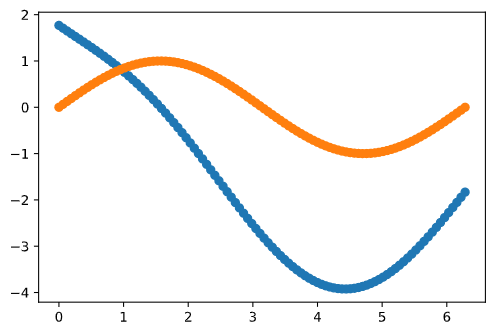
\includegraphics[width = 0.7\columnwidth]{figure/caseCalcKinv.png}
					\caption{逆行列を直接数値計算によって計算した場合}
				\end{minipage}
					\begin{minipage}{0.5\hsize}
					\centering
					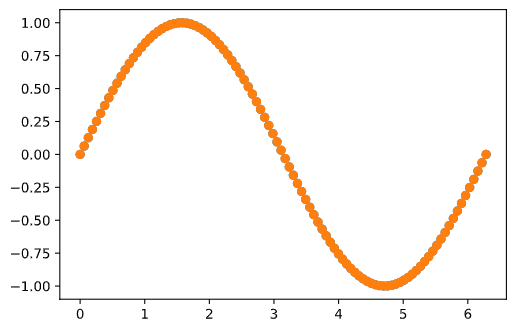
\includegraphics[width = 0.7\columnwidth]{figure/caseCalcLinearEq.png}
					\caption{$ \bd{K} \bd{a} = \bd{y} $を,$ \bd{a} $について解くことによって計算した場合}
				\end{minipage}
			\end{figure}
			左に示すのは,直接計算する場合,右に示すのは線型方程式を解く場合である.2つには大きく差が出ているが,この差は数値計算解法の差にある.すなわち,このような場合は陽に逆行列を求めるのではなく,線型方程式を解くことによって得ることを考える.
		\subsection{尤度関数の最大化について}
			尤度関数が$ \bd{y} $に対して最大化するとき,この問題はシンプルな二次形式:$ -\bd{y}^T \bd{K}^{-1} \bd{y} $の最大化する問題となる.
			
			ある二次形式$ \bd{y}^T \bd{A} \bd{y}$の値は,$ \bd{A} $が半正定値行列であるならば,その最大値,最小値は最大・最小固有値と一致すると知られている.また,$ \bd{A}^{-1} $の固有値は,$ \bd{A} $の固有値の逆数をとることが知られている.すなわち,尤度関数の最大化は,$ \bd{K} $の固有値$ \lambda_{K,i} $を用いて,$ \bd{y}^T \bd{K}^{-1} \bd{y} - \frac{1}{\lambda_{K,\max}} $という制約条件に帰結できる.この,制約条件を計算する際には,$ \bd{K} \bd{a} = \bd{y} $を解き,$ \bd{y}^T \bd{a} $を計算することで,逆行列を陽に計算せずに済む.
			
		\subsection{取り組んだこと}
			最初は,$ \bd{y} = \bd{K} \bd{a}$と表した上で,固有値の線形和で$ \bd{a} $で表されることから,この重みを最適パラメータと考え,最適化問題へ落とし込むことを考えた.しかしながら,$ \omega_{\eta} <\kappa$の不等式制約があり,これを破られると計算が破綻してしまうという問題が発生しておりました.ラグランジュ乗数法における不等式制約や,バリア関数による不等式制約表現を考えましたが,なかなかうまくいきませんでした.したがって,直接$ \bd{y} $を設計しようと試みております.
			すなわち,$\omega_{\eta} = \kappa \frac{2}{\pi} \tan^{-1} \sum_i a_i e_i $とRitz法を応用して表したりすることで,不等式制約を必ず満たすようにするように,関数表現をうまく設定してやることで,不等式を回避する.
		\subsection{母線長の最適化}
			どのように母線を最適化するか:ポテンシャルエネルギー?問題を二つに分割することで,目的関数のみの最適化問題を2つ解けばよいというシンプルな問題になる.など,
	\section{荒井先生コメント}
		以下の件、厳密な意味での1はすぐには思いつきませんが2については多くの軍事応用が必死にやられています。
		例えば、戦車の装甲、特に砲頭部は、相手の砲弾が当たっても食い込んでくること無くはじく(それた方向に反射させる)ように形状設計されています。まさに幾何数学の塊のような研究が昔からなされてきました。この軍事応用の世界的に有名な数理研究所がオランダにあります。
		
		今、私のパソコンは昔のもので検索能力に欠けるので情報を入手できませんが一昔前にいくつか公開された研究があった気がします。弾が当たって弾かれる動画もあったような。
		
		後、新幹線の新型車両の空気抵抗とかは、日立が公開していたと思います。
		レーシングカーの空気抵抗についてはホンダやトヨタがあるかと思います。
		君の研究に近いところではスイムスーツの流体抵抗もあるかと。これは素材も絡むか。
		
		今、リラックスしすぎていて中々頭が働いていないのですぐに思いつかないのをお許しください。
		とりあえず。
	\section{To Do List}
		\begin{itemize}
			\item 論文流れについて考え始める
			\item プログラムデバッグ続き
		\end{itemize}
				
	\newpage
\vspace{10cm}
%%%%%%%%%%%%%%%%%%%%%%%%%%%%%%%%%%%%%%
% 3.達成できなかったこととその問題点
	%\articleSPRthree
	
%%%%%%%%%%%%%%%%%%%%%%%%%%%%%%%%%%%%%%

\vspace{14cm}
%%%%%%%%%%%%%%%%%%%%%%%%%%%%%%%%%%%%%%
	\articleSPRfour
	\articleSPRfive
\end{document}
